% !TEX root = ../main-ring-signature.tex

Ring signatures, introduced by Rivest, Shamir and Tauman, \cite{AC:RivShaTau01}, allow to anonymously sign a message on behalf of a ring of users $R=\{P_1,\ldots,P_n\}$, only if the signer belongs to that ring. That is, no one outside $R$ can forge a valid signature and  an honestly computed signature reveals no information about the actual signer.  
Unlike other similar primitives such as group signatures \cite{EC:ChaVan91}, ring signatures are not coordinated: each user generates secret/public keys on his own --- i.e.~no central authorities --- and might sign on behalf of a ring without the approval or assistance of the other members.

The original motivation for ring signatures was anonymous leakage of secrets. Suppose a high rank officer wants to leak some sensitive document to a journalist without revealing its identity. To do so, it signs this document using a ring signature where the ring contains all other high rank officers. The journalist is convinced that some high rank officer signed the document, but it has no clue who.

Besides this hypothetical application, with the advent of cryptocurrencies, ring signatures have found new and more practical applications. For example, for spending a coin in Monero, a user form a ring from public keys in the blockchain to issue a ring signature on the transaction. Thereby, the anonymity properties of the ring signature guarantee untraceability and fungibility. 
Given the practical usefulness of ring signatures, it becomes crucial to study and improve its efficiency.

\subsection{Related Work}
The efficiency of a ring signature might be splitted in three parameters: the signature size, the cost (time) of computing a signature, and the cost (time) of verifying a signature. Among these metrics, the signature size has received the most attention and improvements in the size usually imply improvement on the other metrics.
In terms of ring size, one the most efficient constructions have signature size logarithmic in the size of the ring \cite{EC:GroKoh15,EC:LLNW16}. Both constructions rely on the {random oracle model}, which is an idealization of hash functions with known theoretical inconsistencies \cite{FOCS:GolKal03}. Malavolta et al.~constructed a constant size ring signature without random oracles \cite{AC:MalSch17} using SNARKS \cite{EC:GGPR13,AC:DFGK14,EC:Groth16} as a subroutine, which are known to require controversial non-falsifiable assumptions such as the knowledge of exponent assumption  \cite{STOC:GenWic11,C:Naor03}. Unlike traditional falsifiable assumption (e.g.~DDH), is not possible to efficiently check whether the adversary effectively breaks the assumption as it require the non-existence of some efficient extractor. In practice, random oracles and non-falsifiable assumptions offer great efficiency at the price of less understood security guarantees. Therefore, it is still interesting and challenging to explore practical constructions from more standard assumptions.

Using only standard assumptions (RSA), Chase and Lysyanskaya proposed a ring signature scheme whose size is independent from the number of users \cite{C:ChaLys06}. Unfortunately , the size too large for consider it practical.
%\footnote{This works seems to has gone unnoticed in the ring signature literature. In fact, to the best of our knowledge, the only recent work citing it is \cite{AC:MalSch17}.} 
The main contribution of their work are
signatures of knowledge, which they use as primitive to construct ring signatures from accumulators, following Dodis et al.~\cite{EC:DKNS04}. The scheme description is only sketched and no proof of security is given but, for fairness (as also noted in \cite{AC:MalSch17}), their work is previous to the (now standard) formal definition of ring signatures of Bender et al.~\cite{TCC:BenKatMor06}. Their scheme goes as follows.
Given a ring of RSA public keys $R = \{(N,y_1),...,(N,y_n)\}\subseteq \Z_{\phi(N)}$, one can compute an accumulated value $a = g^{\prod_{i=1}^n y_i}$ and a witness $w_i = a^{-y_i} \mod N$ that $y_i$ is accumulated in $a$, which can be verified checking if $a = w_i^{y_i} \mod N$. A ring signature on a message $m$ is computed as a signature on $m$ of knowledge of $x_i,y_i\in \Z_{\phi(N)}, w_i\in \Z_N$ such that: a) $x_iy_i = 1 \mod \phi(N)$ and b)  $a = w_i^{y_i} \mod N$. However, signatures of knowledge are built on top of simulation sound NIZK which in turn is built from standard NIZK, and the only NIZK proof system for a) and b) seems to be generic NIZK for circuit satisfiability. For example, using Groth-Sahai proofs the proof will require $O(|C|)$ elements of a bilinear group, where $|C|$ is the size of the circuit for computing a) $\wedge$ b). One might expect the circuit for a) and b) to have at least $\approx 10^4$ gates\footnote{For example, in \url{https://www.cs.bris.ac.uk/Research/CryptographySecurity/MPC/}, a circuit for multiplying 32x32-bit integers requires $\approx 10^4$ gates. Our estimation is quite conservative since RSA integers should be of size $\geq 1024$, and further, one might expect a circuit for a) and b) to contain at least thousands of multiplication gates.}, and thus the proof will be of size greater than $10^4$ elements of a bilinear group. %We would like to note that the NIZK proof used in this construction is \emph{non-blackbox}, that is, it requires a bit-by-bit representation of elements and group operations of $\Z_{\phi(N)}$ and $\Z_N$. We believe this 

Despite Chase and Lysyanskaya's construction, without random oracles or non-falsifiable assumptions all constructions have signatures of size linear in the size of the ring, being the sole exception the $\Theta(\sqrt{n})$ ring signature of Chandran et al.~\cite{ICALP:ChaGroSah07}. They construct a simple and elegant ring signature which at its core implements a \emph{set-membersip proof}, i.e.~a proof that somme commited public key belongs to the set of public keys of the ring users. Their set-mebership proof is quite strong, in the sense that the verification keys may be even chosen by the adversary. Going a step forward, we will build a more efficient but weaker set-mebership proof which is still useful for building ring sinatures.

We note that no improvements in the
signature size have been made within a decade. In fact, although two previous works claim to construct signatures of constant \cite{ACISP:BosDasRan15} or logarithmic \cite{IET:GriSusPla16} size, in Appendix \ref{sec:rs-flawed} we show that one construction fails to give a correct proof of security and the other is in fact of size $\Theta(n)$. The only (non-asymptotic) improvements we are aware of are \cite{TCC:Rafols15,AC:GonHevRaf15}.

\subsection{Our contribution}
In this work we present the first ring signature based on bilinear groups whose signature size is asymptotically smaller than Chandran et al.'s, and whose security is proven under falsifiable assumptions and without random oracles. Our ring signature consists of $\Theta(\sqrt[3]{n})$ group elements, computing a signature requires $\Theta(\sqrt[3]{n})$ exponentiations, and verifying a signature requires $\Theta(n^{2/3})$ pairings. Our ring signature is perfectly anonymous, i.e.~it completely hides the identity of the actual signer, and is computationally infeasible to forge signatures for non-members of the ring. A comparision of our ring signature and Chandran et al.'s is given in Table \ref{table:eff}

The security of our construction relies on a security assumption --- the {permutation pairing assumption} --- introduced by Groth and Lu \cite{AC:GroLu07} in an unrelated setting: proofs of correctness of a shuffle. While the assumption is ``non-standard'', in the sense that is not a ``DDH like'' assumption, it is a falsifiable assumption and it was proven hard in generic symmetric bilinear groups by Groth and Lu. We work on asymmetric groups (Type III groups \cite{EPRINT:GalPatSma06}) and thus we give a natural variant of the permutation pairing assumption which we also prove secure in generic asymmetric bilinear groups.

%Our ring signature outperforms Chandran et al.'s in terms signature size for any $n > 144$, in terms of signature generation time for any $n>96$, and in terms of verifier efficiency for any $n>111$. However, this analysis should be taken with care, since Chandran et al.'s signature is proven secure under the decisional linear (DLin) assumption while ours is proven secure under the permutation pairing assumption. Being the permutation pairing assumption much less studied than DLin, it could be the case that our scheme would be as secure as Chandran et al.'s at higher values of the security parameter. In Table \ref{table:eff} we provide a comparison between our scheme and Chandran et al.'s.
 
% !TEX root = ../main-ring-signature.tex

\begin{table}[h]
\begin{center}
\begin{minipage}{\textwidth}
\begin{center}
%\begin{scriptsize}
\begin{tabular}{l|l|l}
%\hline
                                           & Chandran et al.~\cite{ICALP:ChaGroSah07} & This work \\
\hline%\hline
\rule{0pt}{2.5ex}CRS size  $\GG_1/\GG_2$              & 4/4                                      & $4/4$       \\
\rule{0pt}{2.5ex}Verification key size $\GG_1/\GG_2$    & $1/0$                                       & $2/5$       \\
\rule{0pt}{2.5ex}Signature size      $\GG_1/\GG_2$      & $12\sqrt{n}+10/15\sqrt{n}+8$                        & $24\sqrt[3]{n} + 36/34\sqrt[3]{n} + 24$\\
\rule{0pt}{2.5ex}Signature generation time & $37\sqrt{n}+23$                        & $80\sqrt[3]{n}+71$\\
\rule{0pt}{2.5ex}Verification time         & $2n + 60\sqrt{n}+38$                & $8n^{2/3} + 162\sqrt[3]{n} + 118$\\
%\hline 
\end{tabular}
%\end{scriptsize}
\end{center}
\caption{Comparison of Chandran et al.'s ring signature and ours for a ring of size $n$. 'Signature generation time' is measured in number of exponentiations, 'Verification time' is measured in number of pairings, and all other rows are measured in number of group elements.\label{table:eff}}
\end{minipage}
\end{center}
\end{table}


We require members of the ring to erase the random coins after generating the public/secret key pair. The reason is that the public keys contain group elements whose discrete logs are of the form $(a,a^2)$. Although this helps to embed an instance of the permutation pairing assumption in the set of (honest) public keys, it prevents oblivious sampling of the verification keys. Thereby, users must generate information that, when corrupted by the adversary, renders easy the permutation pairing assumption. We remark that this only affects unforgeability and honestly generated signatures still don't reveal any information about the signer.

Nevertheless, even without erasures, it is unlikely that such adversary exists. We uphold this on the fact that our scheme is secure, without erasures, under a stronger assumption, the \emph{interactive} permutation pairing assumption, which we prove secure in generic bilinear groups.
%
%\begin{figure}[!t]
%	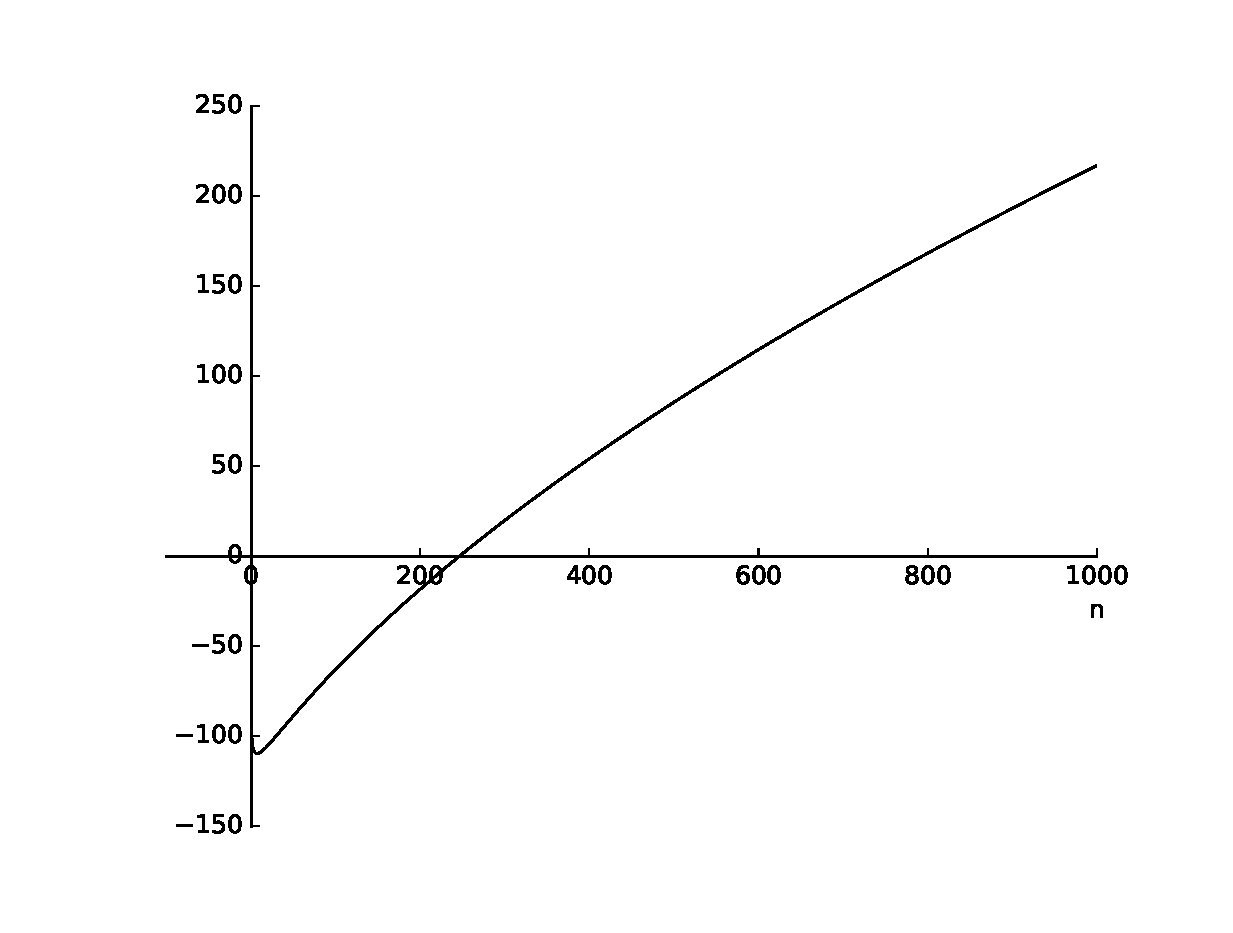
\includegraphics[scale=.25]{intro/sign_size}
%	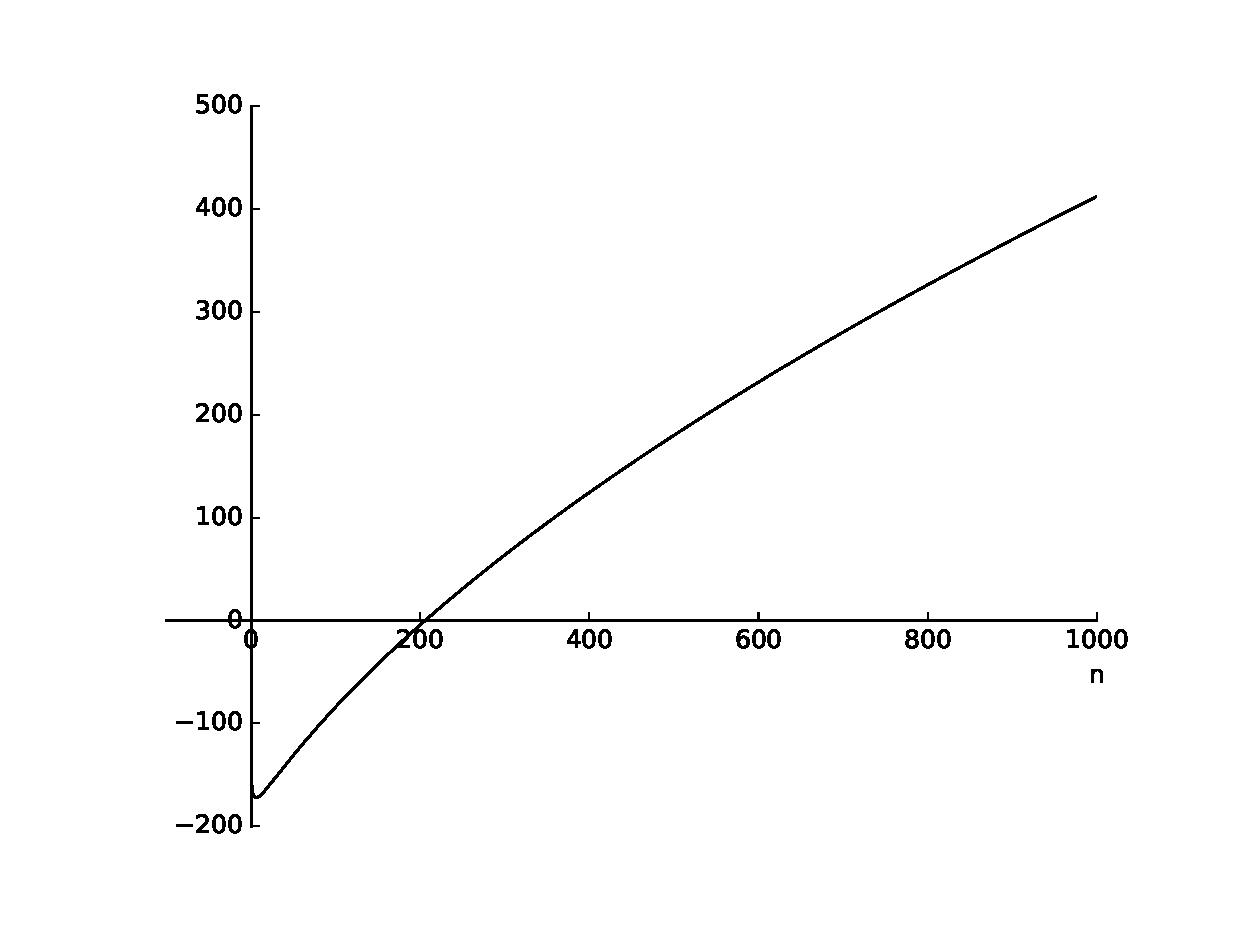
\includegraphics[scale=.25]{intro/sign_time}
%	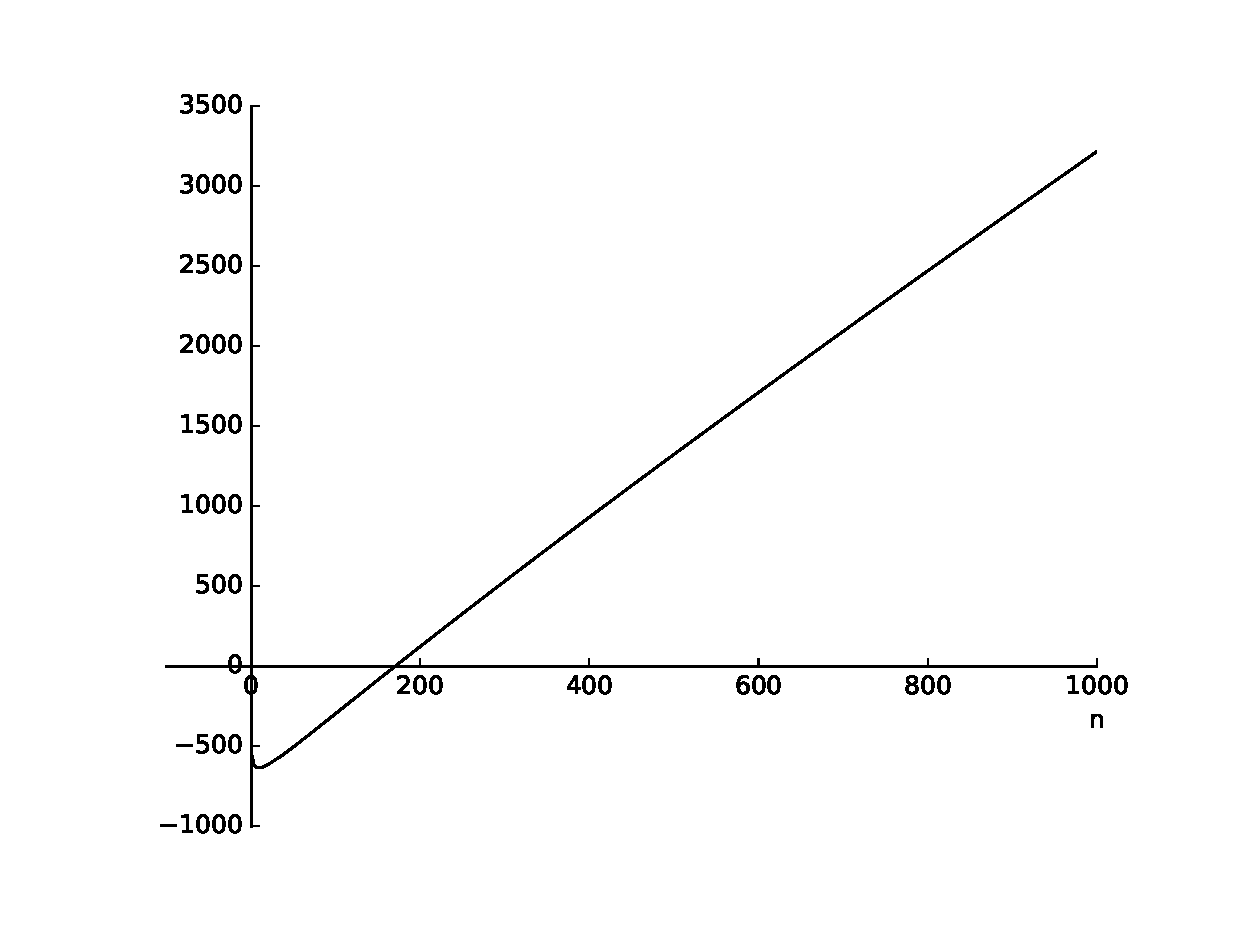
\includegraphics[scale=.25]{intro/ver_time}
%\end{figure}
